\documentclass[conference]{IEEEtran}
\IEEEoverridecommandlockouts
% The preceding line is only needed to identify funding in the first footnote. If that is unneeded, please comment it out.
\usepackage{cite}
\usepackage{amsmath,amssymb,amsfonts}
\usepackage{algorithm}
\usepackage{algorithmicx}
\usepackage{algpseudocode}
\usepackage{tikz}
\usetikzlibrary{arrows.meta, positioning}
\usepackage{listings}
\usepackage{graphicx}
\usepackage{textcomp}
\usepackage{xcolor}

\graphicspath{{../images/}}
\def\BibTeX{{\rm B\kern-.05em{\sc i\kern-.025em b}\kern-.08em
    T\kern-.1667em\lower.7ex\hbox{E}\kern-.125emX}}
\begin{document}

\title{Singular Value Decomposition and Principle Component Analysis}


\author{\IEEEauthorblockN{Edwin Sarver}}

\maketitle

%TODO: https://tex.stackexchange.com/questions/13675/use-graphviz-within-tex

\section{Introduction}
Singular Value Decomposition (SVD) and Principle Component Analysis (PCA) are 
mathematical algorithms that allow, primarily, for the simplification of data.
This project implemented a command-line application to compress an image by 
using SVD. PCA was used to analyze a data-set comparing the genetic markers that
may determine the type of Leukemia a patient may have. 

\section{Algorithms}\label{algo}
Two main algorithms were used in this project: Singular Value Decomposition (SVD)
and Principle Component Analysis (PCA).

\subsection{Singular Value Decomposition (SVD)}
Singular Value Decomposition is a mathematical method that uses Linear Algebra
techniques to separate a matrix into the parts that are most mathematically 
important. A given matrix $M$ can be separated into three matrices $U$, 
$\Sigma$, and $V$.

%TODO describe U, Sigma, and V and what they mean.

\subsubsection{Theoretical Performance}
The purpose of the SVD algorithm in this project was to produce a compressed image. 
The implementation did not need to be fast. The performance of the algorithm was, 
therefore, determined by the space-efficiency of the file that was output. 

%TODO add Theoretical analysis of space efficiency
The theoretical space efficiency for the implemented program is 
\begin{itemize}
	\item 3 longs (64-bits each)
	\begin{itemize}
		\item 1 for height of the image
		\item 1 for width of the image
		\item 1 for rank
	\end{itemize}
	\item 1 char for the maximum gray-scale value
	\item 16-bits for each item in $U$, $\Sigma$, and $V$
\end{itemize}

The number of elements in $\Sigma$ will be equal to the rank of the image. 
The number of elements in the $U$ matrix will be the rank times with height of the image.
Similarly, the number of elements in the $V$ matrix will be the rank times the width of the image.

Therefore, the compression of the image will be proportional to the rank selected by the user for 
a given image. 

The theoretical size of the image is shown in Equation \ref{compression}

\begin{equation}
\label{compression}
		3*8 + 1 + 2*rank*(height + width + 1)
\end{equation}

%TODO Theoretical error analysis
The theoretical error for each image will depend on the image itself. This information, however, can 
be found in the singular value matrix, $\Sigma$. If the rank is $k$, the error in the approximation 
will be the element at $k+1$ in the diagonal of $\Sigma$ (i.e. the element at $(k+1, k+1)$).

\subsubsection{Experimental Performance}

%TODO add Experimental analysis of space efficiency
As expected, the space used for a given image increases proportionally as the rank increases
as shown in Figure \ref{size_vs_rank}.

\begin{figure}
	\centering
	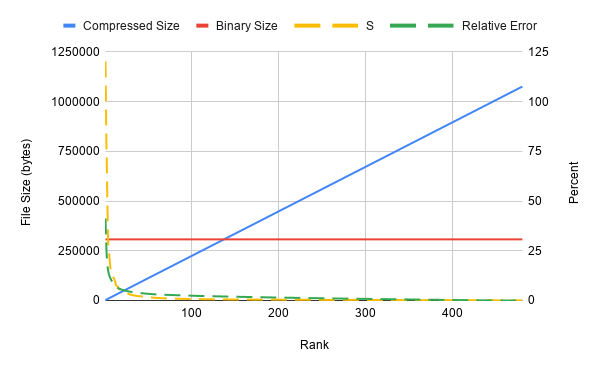
\includegraphics[width=3.25in]{compression.png}
	\caption{File Size vs Rank}
	\label{size_vs_rank}
\end{figure}

%TODO Experimental error analysis
The approximation error is also shown in Figure \ref{size_vs_rank} as the dotted lines. The actual
error is very close to the theoretical error, but because the compressed image was stored as a 
half-precision float, the error does tend to be a little different.

\subsection{Principle Component Analysis (PCA)}
Principle Component Analysis simplifies the analysis of multi-dimensional data-sets by 
reducing the dimensionality of the data. This makes data visualization easier by finding
which dimensions of the data have the greatest impact on the categorization of the data. 

Reducing the dimensionality of data is important when a given problem may have many possible
related factors such as in the realm of genetics. In our project we studied the factors that 
be related to 2 different kinds of Leukemia, Acute Lymphoblastic Leukemia (ALL) and Acute Myeloid
Leukemia (AML). 

In order to process the data, it must be set up with rows being the observations and the columns 
being the variables. We then calculate the matrix $B$ so that the mean of each column is subtract 
from it's constituent parts. The co-variance matrix can then be calculated by $S=B^T B/(n-1)$.

$S$ can then be decomposed into eigenvectors and eigenvalues ($V$ and $D$ respectively) such that 
$S = V D V^T$. This is the same as SVD, except that the matrix $U = V$.

The $D$ matrix shows the relative strength of the components that are represented by the columns
in the $V$ matrix.

By choosing the top 2 or 3 principle components (the highest values in $D$), the corresponding 
weights in the $V$ matrix can then be used to plot the original observations. This will cause 
value to clump and thus categorization of the data becomes much easier.

After applying PCA on the Leukemia data-set, the ALL and AML data is easier to categorize due to
the separation between the data-points, as shown in Figure \ref{pca}. There is clear separation 
between the points in the lower left and the upper right of the graph. 

\begin{figure}
	\centering
	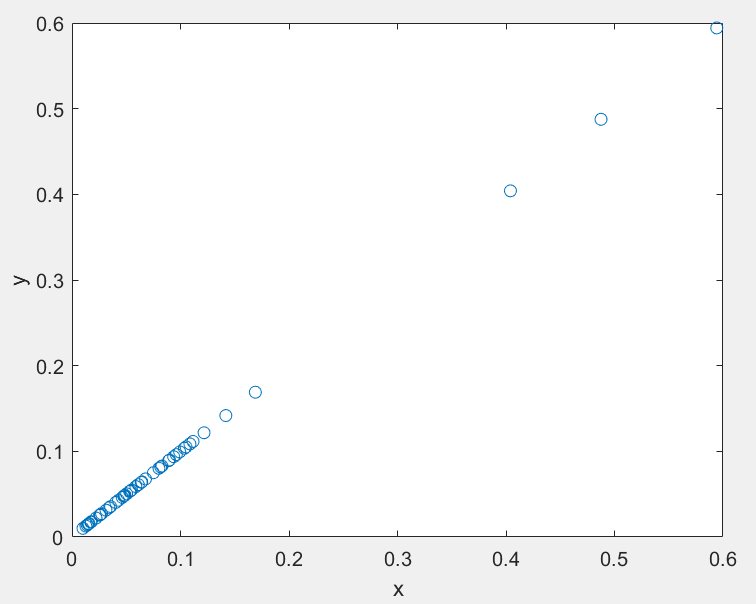
\includegraphics[width=3.25in]{PCA_1.png}
	\caption{File Size vs Rank}
	\label{pca}
\end{figure}

\section{Insights}
%TODO Efficiency, modularity, generalizablility, stability, etc. 
The modularity and generalizability of SVD and PCA make them valuable for 
many applications. Static image compression is just one of the many possible
ways that SVD can be utilized. Another application is for video compression by
taking the difference between frames and then compressing the resulting difference.
Any application that requires the compression or analysis of highly-dimensional data
can be a possible application for SVD and, in the case of analysis, PCA. 


\section{Test Cases}
In this project, many forms of testing were utilized to test the image processing implementation: Unit tests, correctness tests,
and performance tests.

\subsection{Unit Tests}
Unit tests were used to ensure that each part of the program functioned as intended even after
changes were made to the code base. Included in these tests were tests to verify the algorithms
described in section \ref{algo}. The PGM images used in the unit tests were very small and were
only large enough to ensure that the basic functionality of the SVD algorithm was correct.  


\subsection{Correctness Tests}
Correctness tests for the SVD implementation were manual because they required the analysis of images.
The image used to verify the correctness of the algorithms was the provided image of the College of 
Arts and Sciences building on the University of Akron campus. In the course of testing, several issues
were identified and corrected. Most of the issues that were identified arose from incorrectly calculating
the position in the matrix that a particular element in the compressed, binary image file should occupy. 

\subsection{Performance Tests}\label{perf_explanation} %TODO revisit this
Performance test were also manual. An image of Saturn was downloaded from \cite{b2}.
The image was translated into a binary representation, then the original pgm was split 
into a header and data file with a python script. The split files were then compressed 
using the SVD compression algorithm across all possible ranks. The resulting binary 
files were then compared against the binary files that were generated directly from the 
original PGM files for size. The compressed files were then uncompressed to pgm files 
and were inspected for visual fidelity and the error from the original image was 
calculated. The relative error for each rank on each image could therefore be calculated.
The images at various stages of approximation are shown in Figures \ref{svd1}, \ref{svd91}, 
and \ref{svd480}.


\begin{figure}
	\centering
	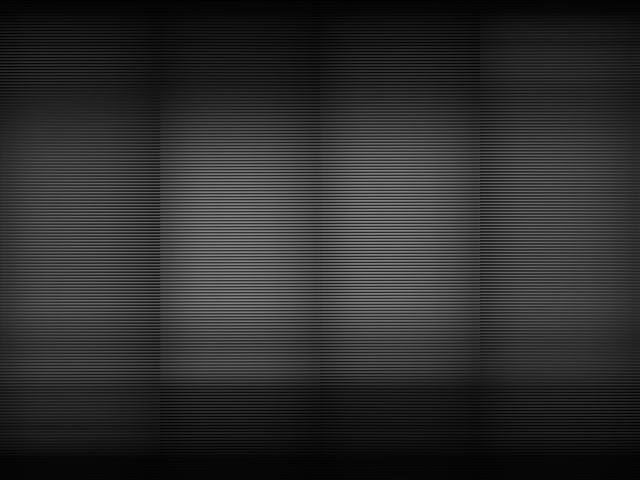
\includegraphics[width=3.25in]{saturn_SVD_1.png}
	\caption{SVD approximation at Rank 1}
	\label{svd1}
\end{figure}

\begin{figure}
	\centering
	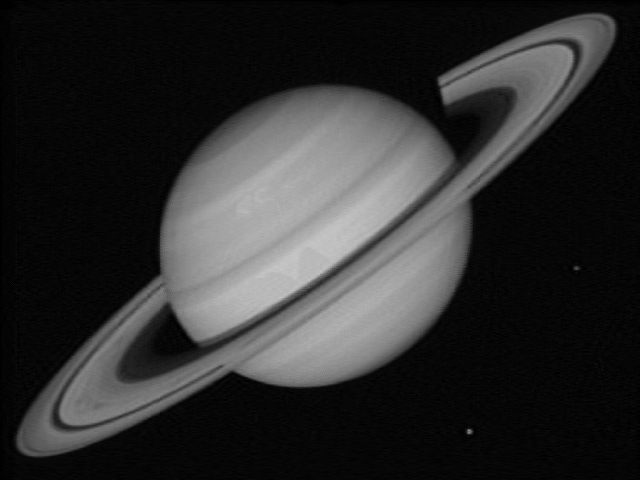
\includegraphics[width=3.25in]{saturn_SVD_91.png}
	\caption{SVD approximation at Rank 91}
	\label{svd91}
\end{figure}

\begin{figure}
	\centering
	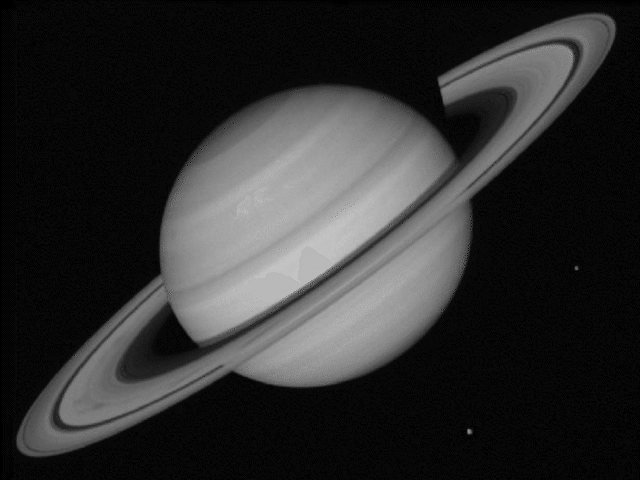
\includegraphics[width=3.25in]{saturn_SVD_480.png}
	\caption{SVD approximation at Rank 480}
	\label{svd480}
\end{figure}

The relative error can also be calculated from the singular values in the $\Sigma$ matrix.
The program was therefore modified to print the singular values to a separate file for further
analysis.

%\subsection{Design}
% TODO
%\subsection{Results}
% TODO

\section{Conclusion}
Singular Value Decomposition is a highly generalizable, powerful algorithm that creates a simplified 
mathematical representation of a data-set that describes which components are most important to the 
overall representation of the data-set. This allows for image compression by removing less important 
components of the image, but also allows for data analysis by the same mechanism when used in Principle
Component Analysis.  


\begin{thebibliography}{00}
	\bibitem{b1} T. H. Cormen, C. E. Leiserson, R. L. Rivest, and C. Stein, Introduction to Algorithms, 3rd ed., The MIT Press, 2009, pp. 594--602, 709--731 
	\bibitem{b2} "PGMA Files," fsu.edu, Jun 10, 2011. [Online]. Available: https://people.sc.fsu.edu/~jburkardt/data/pgma/pgma.html. [Accessed: Nov. 11, 2019].
\end{thebibliography}

\end{document}
